
\documentclass[letterpaper, 10 pt, conference]{ieeeconf}  % Comment this line out if you need a4paper

%\documentclass[a4paper, 10pt, conference]{ieeeconf}      % Use this line for a4 paper

\IEEEoverridecommandlockouts

\overrideIEEEmargins                                      % Needed to meet printer requirements.

%In case you encounter the following error:
%Error 1010 The PDF file may be corrupt (unable to open PDF file) OR
%Error 1000 An error occurred while parsing a contents stream. Unable to analyze the PDF file.
%This is a known problem with pdfLaTeX conversion filter. The file cannot be opened with acrobat reader
%Please use one of the alternatives below to circumvent this error by uncommenting one or the other
%\pdfobjcompresslevel=0
%\pdfminorversion=4

% The following packages can be found on http:\\www.ctan.org
%\usepackage{natbib}
\usepackage{graphicx} % for pdf, bitmapped graphics files
\graphicspath{ {images/} }
%\usepackage{epsfig} % for postscript graphics files
\usepackage{mathptmx} % assumes new font selection scheme installed
\usepackage{times} % assumes new font selection scheme installed
\usepackage{amsmath} % assumes amsmath package installed
\usepackage{amssymb}  % assumes amsmath package installed
\usepackage[mathscr]{euscript}

\title{\LARGE \bf
Increasing Quadrotor Endurance Through Momentum Analysis
}


\author{Alexander B. Faustino and Timothy Bretl% <-this % stops a space
	\thanks{The authors are with the Department of Aerospace Engineering, Coordinated Science Laboratory, 
		University of Illinois at Urbana-Champaign, Champaign, IL 61801, USA
		\tt\small \{afausti2, tbretl\}@illinois.edu}%
}


\begin{document}

\maketitle
\thispagestyle{empty}
\pagestyle{empty}


%%%%%%%%%%%%%%%%%%%%%%%%%%%%%%%%%%%%%%%%%%%%%%%%%%%%%%%%%%%%%%%%%%%%%%%%%%%%%%%%


\begin{abstract}
	A problem that continues to persist for quadrotor UAVs is their low endurance relative to other prominent UAV platforms. There exist three main approaches to solving this problem: improving hardware efficiency, designing new hybrid systems, and developing software solutions that focus on optimal planning and control. Of the three, software solutions have received the least attention. Existing methods are either heavily constrained, challenging to implement on physical systems, or require significant off-line computation. In this paper we present a method for finding power minimal, smooth trajectories for a quadrotor in SE(3) using exiting models for power and energy consumption. We show that the problem can be formulated as a constrained, continuous time optimal control problem with a polynomial cost function that can be solved numerically. Through simulation we show that our approach, when compared to existing methods, reduces total energy consumption by \textbf{INSERT RESULTS HERE}\% on average. 
\end{abstract}

\section{INTRODUCTION}
 
The last decade has seen quadrotor helicopters explode in popularity. From an emerging unmanned aerial vehicle (UAV) concept to a prominent research and commercial platform \cite{kumar2012opportunities,hoffmann2007quadrotor} quadrotors have become the nearly ubiquitous aerial robot. Their relative low cost and the simplicity of their dynamics when near hover \cite{bouabdallah2004pid} has made them popular in numerous applications \cite{heng2015efficient,roberts2017submodular,frazzoli2002real}.

The condition of operating near hover also introduces the quadrotor platform's greatest weakness, power efficiency. The power required to keep a quadrotor at hover is approximately 200 W per kg \cite{kumar2012opportunities}. Since quadrotors are rarely flown dynamically far away from hover when used in application, the problem of power efficiency creates a practical limit on their utility. This limit restricts the size of an area that can be explored, the number of images that can be captured by a camera, the mass of potential payloads, etc.. In robotics, maximizing endurance is mostly thought of as a design problem handled by manufacturers. In this paper we present evidence that choices about trajectory and velocity also have a meaningful effect on flight time.

Determining an aerial vehicle's endurance is a common problem in flight mechanics. Solutions for fixed wing and rotor aircraft maximum endurance in steady, forward flight are well known and widely used \cite{anderson2005introduction,leishman2006principles}. Maximum endurance is achieved by traveling at the relative velocity, $V_\infty$, where the power required, $P_{req}$, to overcome the drag force, $D$, is at a minimum. We call this velocity $V_{me}$. 


\begin{figure}[ht]
    \label{QuadDiagram}
	\centering
	
\includegraphics[width=8cm]{placeholder-image.jpg}
	\caption{Coordinate system and flow diagram illustrating induced velocity, force balance at equilibrium, etc..}
\end{figure}


\section{Related Work}

\subsection{Existing white box models}
White box models for quadrotor power consumption are derived from theoretical models for general rotorcraft, mainly presented by Leishman \cite{leishman2006principles}. Leishman's full model has aerodynamic power required for a steady maneuver equivalent to the sum of induced power, parasitic power, profile power, and power required to climb. Aerodynamic power is then scaled by an efficiency factor to convert to electrical power consumed. The individual power terms can be approximated, simplified, or assumed negligible to reduce model complexity. Which of these terms is included and how they are simplified is the main difference between the existing white box models implemented specifically for quadrotors. 

A nearly comprehensive model for power consumption is given by Liu et al. \cite{liu2017power}. Their model contains three of the four terms from Leishman's model relevant to quadrotors: induced, profile, and parasitic, while neglecting the power required to climb. Somewhat similar to the black box models, their model requires initially collecting flight data to numerically determine seven constants. Their model is validated by flying a known trajectory and comparing the estimate of power to the actual power measured onboard. Our experiments are a natural extension to this validation, as we fly similar trajectories with more parameter variation. What differs is that we analyze how the individual terms contribute to the estimate's accuracy rather than just determining the accuracy.

In \cite{bangura2012nonlinear} Bangura and Mahony present a model for mechanical power produced by the rotors as the integral part of their nonlinear dynamic model. They draw on the previous work by \cite{leishman2006principles} and \cite{hoffmann2007quadrotor} to derive a model that more accurately depicts the relationship between the rotors' mechanical and aerodynamic characteristics and the dynamics of the whole body during aggressive maneuvers. While this model has seen success in implementation, the traditional thrust-and-torque-based nonlinear model is still the most prevalently implemented.

\subsection{Trajectory optimization}
Ware and Roy \cite{ware2016analysis} incorporate urban wind data to find more efficient trajectories between two points in the urban canopy layer. Using the wind's prevailing speed and direction above the surrounding buildings as the input to a CFD solver, they generate a grid with 1 m resolution. Similar to \cite{di2015energy} they create a graph for a fixed altitude such that each interior node has eight edges. Using the wind vector, $v_w$, from the CFD solution, they can then choose an upper and lower bounded ground velocity, $v_g$, for the quadrotor such that it minimizes:
\begin{align*}
E_i = \frac{T(v_i + v_\infty \sin{\alpha}) (v_g - v_w) \|d\|}{v_g}
\end{align*}
where $\|d\|$ is the Euclidean distance between the two nodes. They address the acceleration problem encountered by \cite{di2015energy} by constraining the change in velocity, $\Delta v_g$, between edges. Their simulation results show that wind aware planning uses less power than wind naive planning and highlights the importance of having an estimate of the local wind field. We see in the expression for energy consumption that they are only using the dragless model or $P_{ind}$ to minimize power along an edge. We show in Section \ref{sec:Results} that including more terms in their power model, specifically a term for parasitic power, could improve their results.








\section{Flight Mechanic Preliminaries}
\label{flightMechSec}
\label{derivations}
In this section we review the flight mechanic principles necessary for understanding our work. We show derivations for calculating the following: \begin{enumerate}
    \item $P_{req}$ - the power required to maintain level flight 
    \item $V_{mp}$ - the linear velocity where $P_{req}$ is minimized.
    \item $P_{req_{turn}}$ - the power required to maintain a level turn
\end{enumerate} Additionally, we show that for level flight $V_{mp}$ is equivalent to the velocity that maximizes endurance.

\subsection{Power Required $P_{req}$}
Using the standard quadrotor model given in \cite{hoffmann2004stanford} and \cite{pounds2002design} with the coordinate frames illustrated in \ref{QuadDiagram} a simple force balance shows that the pitch angle, $\theta$, can be written as a function of $V$. Assuming a windless environment we can say $V = V_\infty$, the relative velocity of the flow, and write \eqref{ThetaOfV}.

\begin{equation}
    \label{ThetaOfV}
    \theta(V_\infty) = \frac{\rho v_\infty^2 f}{2mg}
\end{equation}

\subsection{Equations Likely Needed}

\begin{equation}
    \label{LevelFlightEqn}
    P_{req} = \frac{k T^2}{2\rho A V_\infty}+(\frac{1}{2}\rho V_\infty^2 S_{ref} C_{D_f})V_\infty
\end{equation}

% \begin{figure}[ht]
% 	\centering
% 	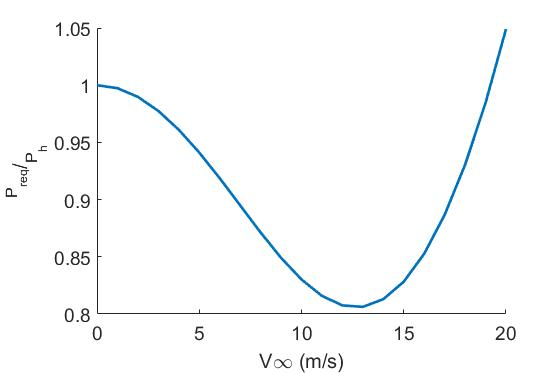
\includegraphics[width=8cm]{constant-config-ratio.jpg}
% 	\caption{The ratio of power required in forward, level flight at a given velocity to power required at hover. Maximum endurance is achieved at the minimum of this curve. For the given configuration we see that flying at $V_{me}$ reduces the power required by 19 percent.}
% \end{figure}

\begin{figure}
    \centering
    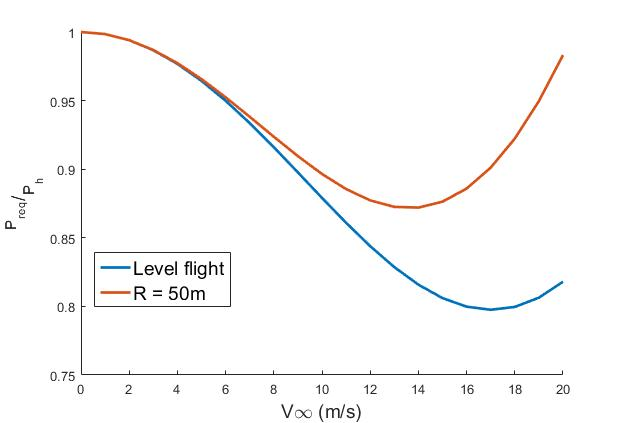
\includegraphics[width=8cm]{images/m100-turn-vs-level.jpg}
    \caption{We compare the theoretical power ratio for our vehicle configuration using momentum theory analysis. If our vehicle was flown straight and level at 17m/s we could expect to fly approximately 21\% longer. Even with losses associated with overcoming centripetal acceleration we can expect to fly 13\% longer by flying at 13m/s while turning with a radius of 50m.}
    \label{m100levelturn}
\end{figure}

\section{Experiments}

To determine the effectiveness of a trajectory, $\mathscr{T}_c$ we empirically compare the time it takes to deplete 1 Ah of charge while flying $\mathscr{T}_c$ versus the time it takes to deplete the same charge at hover. The experiment consists of two main phases: hover flights and trajectory flights where these two phases are flown by the same quadrotor alternately. The parameters defining $\mathscr{T}_c$ (i.e. $v_Q$, $R_t$, type of yaw tracking) vary between iterations while hover parameters remain unchanged. Each iteration begins by replacing the used battery with a fully charged one and determining if local wind speeds are below moderate which we define below. The experiments were designed this way to control for two primary factors, wind and battery variations.

\subsection{Controlling for wind variations}
From equations [eqno?] and decades of aerodynamic research we know that aircraft performance is susceptible to wind disturbances. Extensive work has been done in flight control to reduce wind induced error in the absence of a human pilot. \cite{escareno2013trajectory} and \cite{waslander2009wind} focus on the quadrotor platform while \cite{mcgee2006path} looks at the more traditional fixed-wing aircraft.
In \cite{escareno2013trajectory} and \cite{mcgee2006path} wind disturbance is categorized by 
\begin{equation}
    W = \frac{\lvert V_w \rvert}{\lvert V_Q \rvert}*100\%
\end{equation}
As stated in section \ref{derivations}, in this paper we are not concerned with controlling against moderate or severe wind disturbance. Therefore, before each flight test we measure the local wind speed to ensure $W<20\%$ or below moderate conditions.

\subsection{Mitigating battery issues}


\subsection{Quadrotor platform}
For this experiment we flew the DJI Matrice 100 built to the specifications provided by \cite{sa2018dynamic}. With the exception that we use the Optor visual inertial sensor instead of the discontinued Intel ZR300. All modifications made to their ROS package is available at \textbf{LINK TO GIT}.

\subsection{Measuring consumption}
The DJI SDK reports battery voltage, SoC, and capacity at 10Hz. This was a major reason for selecting this platform as there is no need for additional boards or modules.

\begin{figure}[ht]
	\centering
	
\includegraphics[width=8cm]{placeholder-image.jpg}
	\caption{Graphic detailing setup.}
\end{figure}


\section{CONCLUSIONS}

The results of our experiments are evaluated by assuming two primary use cases for a power consumption model in autonomous UAV planning and control. The first case is predicting the total power consumed by a trajectory, which requires the power consumption model to be accurate across all states in the trajectory. The second case is determining the parameters of minimal power trajectories, where the model’s gradient should have the same sign as the actual power consumed gradient with respect to controllable states. For both cases, our results indicate that a hybrid model based on $v_\infty$ may be necessary.

\subsection{Estimating total power}
As seen in Fig. 4 and Table 1, $P_{ind}$ is by far the largest contributor to accurate estimates of power consumption, especially at lower $v_g$. As expected, the contribution of $P_{par}$ increases with $v_g$, but is still dominated by $P_{ind}$. Interestingly, it is evident that the inclusion of $P_{pro}$ degrades the estimate at greater $v_g$. This could be attributed to the assumption used to neglect a term discussed in \ref{sec:Power} or the method for determining the constant $\kappa_1$. Since all our flights were conducted at near-level flight, it is expected that $P_c$ is nearly negligible.

Table 1 also shows that our full model achieves relative errors lower than previously published models. Since we did not evaluate any of these models using our data, it is not a fair comparison, but it is still worth noting until further verification. This is of particular interest to path and motion planning problems that keep a large margin of battery capacity. By having a better estimate of $P$, uncertainty around max flight time decreases, allowing for a larger feasible trajectory set.

\subsection{Determining minimal power trajectories}
For model-based methods that use gradient descent, it is ideal that the model's computed gradient's descent direction aligns with the descent direction of the underlying physics. Otherwise, the algorithm will converge to non-minimal states. To evaluate this, we approximate the gradient of \eqref{powConsumed} with respect to $v_\infty$, $\theta$, and $\phi$ by taking a finite difference between samples taken while orbiting. In Fig. 4, we see that removing $P_{ind}$ causes discrepancies between the descent directions of $\nabla P$ and $\nabla \hat{P}_{-ind}$. Fig. 4 also shows that this problem diminishes as $v_g$ increases, but as previously stated this magnitude of $v_g$ approaches the current dynamic limit of commercial platforms. Based on that, $P_{ind}$ should always be present in a model where some form of gradient descent is used.

We want to highlight the reliance of our model on accurate estimations of the 3D, time-varying wind field. We think there is room for significant improvement in solutions to this problem, particularly in the atmospheric boundary layer and urban canopies. Looking forward, it will be important to not only estimate the wind vector directly acting on the UAV, like current methods, but to predict the wind field of the entire operating area as well.


%%%%%%%%%%%%%%%%%%%%%%%%%%%%%%%%%%%%%%%%%%%%%%%%%%%%%%%%%%%%%%%%%%%%%%%%%%%%%%%%

%\addtolength{\textheight}{-12cm}   % needs to be before last page to work

%%%%%%%%%%%%%%%%%%%%%%%%%%%%%%%%%%%%%%%%%%%%%%%%%%%%%%%%%%%%%%%%%%%%%%%%%%%%%%%%
\section*{APPENDIX}

Appendixes should appear before the acknowledgment.

\section*{ACKNOWLEDGMENT}

Enter shout outs here.

\bibliographystyle{IEEEtran}
\bibliography{sections/references}

\end{document}
